\section{SRP-PHAT}\label{sec:SRP}
Steered Response Power (SRP) source localization is a method to detect sound source locations using beamforming techniques \cite{krim1996two}. SRP is different from TDOA based methods discussed before. While the generalized cross correlation is a simple cross correlation between each pair of microphones and outputs an estimate of the time delay, the SRP method beamforms the space around the array and computes the energy of each location beam.  It `looks' at all possible directions individually (steering) and computes the power of the signal cross correlation in that direction (beamforming). The assumption is that the cross power of the steered microphone array will be the maximum in the correct source direction. However, the computational demand for this can rise quite fast (depending on the sample rate and the angular resolution of the beamforming), making it nearly impossible to implement in real time applications. But, its performance in difficult conditions outperforms the TDOA based methods \cite{dmochowski2007generalized}. Since real-time localization is not of primary importance for this thesis, SRP based methods can be applied. However, in the same fashion as the GCC methods proposed to pre-filter the signal before performing the cross correlation, PHAT weighing can also be applied on the beamformed signal. The method, called SRP-PHAT, combines the robustness of the SRP to the accuracy of the PHAT. 
\subsection{Steered response power}
The SRP method is based on a regular delay-and-sum beamformer, for a given point in space having range $\rho$, azimuth $\theta$ and elevation $\phi$ with the microphone array, the output of the beamformer is given by
\begin{equation}
    y_{\rho,\theta,\phi}(n)=\sum\limits_{m=0}^{M-1}{w_m x_m[n + f_{0,m}(\rho,\theta,\phi)]},
\end{equation}
where $x_0[n]$ is the signal received at time n, at an arbitrary microphone used as reference, $w_m$ is the amplitude weight for microphone m, and $f_{0,m}(\rho,\theta,\phi)$ is the relative delay between the reference microphone and the $m^{th}$ microphone. When far-field approximation is assumed, the range cannot be computed\footnote{For range computation, the cone approximation cannot be assumed. The delays should be used to compute hyperboloids and not cones. The intersection of the hyperboloids can then be used to compute range. However, it should be remembered that even a small error would lead to large variations in range, as for far-field, small movements in the hyperboloids would cause large movements in range results.} and the delay-and-sum beamformer output can be rewritten as follows:
\begin{equation}
    y_{\theta,\phi}(n)=\sum\limits_{m=0}^{M-1}{w_m x_m[n + f_{0,m}(\theta,\phi)]},
\end{equation}
For $w_m=1$ (assuming perfectly omni-directional and equally sensitive microphones), the output power of the beamformer becomes
\begin{equation}
    \mathbb{E}[{y_{\theta,\phi}(n)^2}]=\sum\limits_{i=0}^{M-1}\sum\limits_{j=0}^{M-1}{R_{x_i,x_j}[f_{i,j}(\theta,\phi)]} \text{, for } i\neq j.
    \label{eq:poweroutputbeamformer}
\end{equation}
This cross correlation is computed in the frequency domain (cross-spectrum) which is then inverse fast Fourier transformed (IFFT).
\begin{equation}
    R_{x_i,x_j}(\tau)= \sum\limits_{k=0}^{N_{f}-1}{X_{i}(k)X_{j}^*(k)e^{j2\pi\frac{k}{N_{f}}\tau}}
\end{equation}

Where $X_{i}(k)$ is the $N_{f}$ (number  point Fast Fourier Transform of a signal from the $i$ microphone.  

\subsection{SRP algorithm}
\begin{itemize}
    \item Compute the cross correlations of the signals received at all the microphone pairs. 
    \item Compute for each set of angles ($\phi,\theta$), the corresponding set of delays for every microphone pair $f_{i,j}(\theta,\phi)$. So if 1$\degree$ angular resolution is used, the SRP method computes delays for 360*180=64800 angular positions, for each microphone pair.
    \item For each ($\phi,\theta$), sum for all microphone pairs, the cross correlation values at the corresponding delays. This sum is the output of the SRP beamformer defined in Eq. \ref{eq:poweroutputbeamformer}\footnote{An improvement on the SRP search algorithm was proposed by pre-mapping the relative delays to their corresponding set of locations \cite{dmochowski2007generalized}. Instead of proceeding with a full sequential search in the 3D space, a search on the possible relative delays, where the cross correlation values are above a threshold, is considered. The possible delays between individual microphone pairs are already known based on the array geometry and can be stored in memory. The computational cost gain can be immense depending on the number of microphones. However, the method is not suitable if the whole acoustic map of an environment in required, so it is not detailed further here.}

%The cross correlations are calculated for each delay subset and related to a set of potential source location in space in the final steps of the algorithm. 
\end{itemize}
\begin{equation}
    S_{SRP}(\theta,\phi)=\sum\limits_{i=0}^{M-1}\sum\limits_{j=0}^{M-1}{R_{x_i,x_j}[f_{i,j}(\theta,\phi)]} \text{, for } i\neq j.\footnote{For a single source, the estimate of the source location from SRP search can be given by:
    $\hat{\phi},\hat{\theta}=\argmax_{\phi,\theta}S_{SRP}(\phi,\theta)$}
     \label{eq:srpSum}
\end{equation}
%\begin{figure}
%    \centering
%    \begin{subfigure}[t]{0.5\textwidth}
%    \centering
%    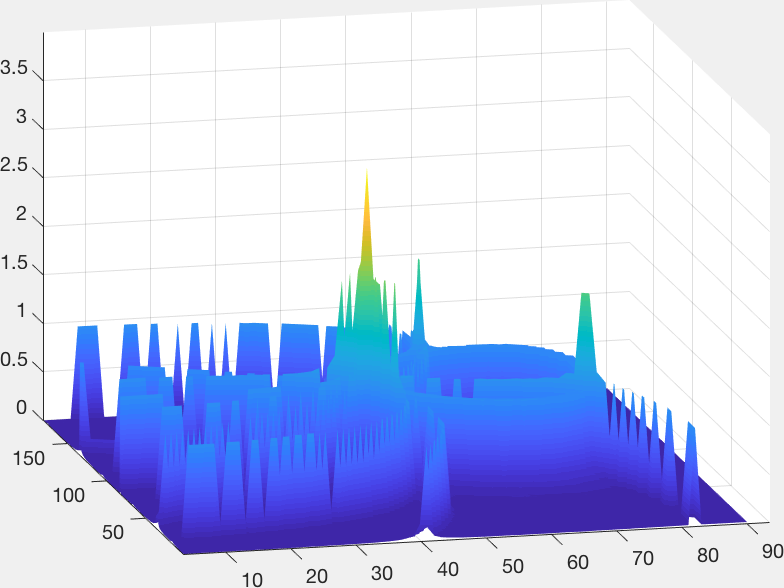
\includegraphics[width=0.9\textwidth]{Figures/viewside.png}
%    \caption{SRP map}
%    \label{fig:viewsidesrp}
%\end{subfigure}%
%\begin{subfigure}[t]{0.5\textwidth}
%    \centering
%    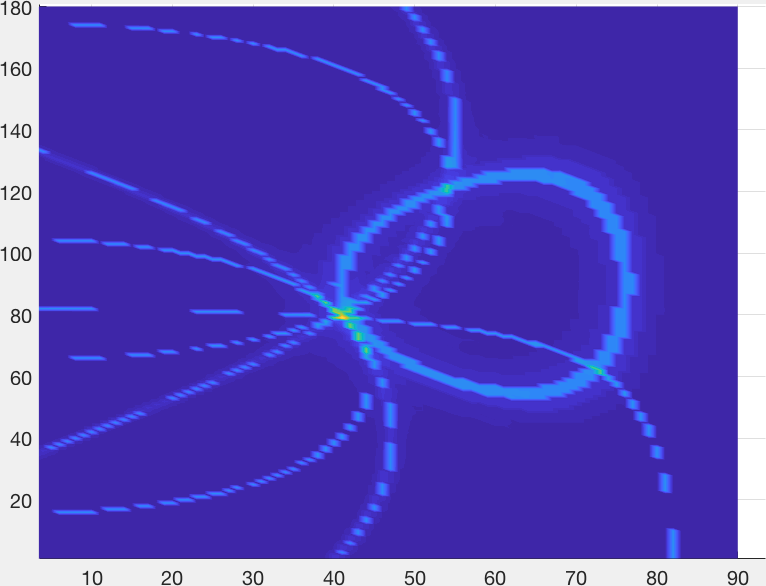
\includegraphics[width=0.9\textwidth]{Figures/topview.png}
%    \caption{SRP heat map}
%    \label{fig:topviewsrp}
%\end{subfigure}
%\caption{Power mapping simulation of source localized using SRP-PHAT algorithm in noiseless, free-field situation. For the simulation, first a 4-channel wav file is created such that the channels contain the same pink noise but delayed between each other. The delays are such that the source would be ideally located at azimuth $80\degree$ and elevation $40\degree$ when localized by a 1m aperture tetrahedral array. SRP-PHAT is then applied on the wav file and power received from different angles (beams) is computed and plotted. As can be seen the algorithm was able to localize the source in these ideal conditions fairly correctly.}
%\end{figure}
%The classical SRP search beamforms sequentially the 3D space and locations [($\phi_{1},\theta_{1}$), ($\phi_{2},\theta_{2}$), ... ,($\phi_{x},\theta_{x}$)] which might be associated with the same relative delay $\tau_{1}$ (in case of a uniform linear microphone array). The cross correlation at delay $\tau_{1}$ is then computed $x$ times, which leads to the same results for each [($\phi_{1},\theta_{1}$), ($\phi_{2},\theta_{2}$), ... ,($\phi_{x},\theta_{x}$)] positions, leading to numerous useless cross correlation computations.
%In GCC methods this issue was taken care of by interpolation, where the microphone pair end-side localization had poor resolution (Fig. \ref{fig:res_diff}). 
\subsection{Extending PHAT to SRP-PHAT}
PHAT can be extended to SRP-PHAT, by simply pre-filtering the cross-correlations before the SRP sum step,
\begin{equation}
    R_{x_i,x_j}(\tau)= \sum\limits_{k=0}^{N_{f}-1}{\psi_{ij}(k) X_{i}(k)X_{j}^*(k)e^{j2\pi\frac{k}{N_{f}}\tau}}
\end{equation}
where
\begin{equation}
    \psi_{ij}(k) = \frac{1}{|{X_{i}(k)X_{j}^*(k)}|}
\end{equation}
%Beamforming techniques for sound localization have been study intensively over the last decades. The main drawback of the conventional beamforming are the side lobes in the localization results. 
% the ideal result is to detect a point precisely at the actual point source location and nothing elsewhere. However that is not the case for SRP-PHAT. For instance, i
\subsection{Localizing with SRP-PHAT}
When localizing a point source using SRP-PHAT, if two microphones are used, the only information that can be computed is the angle of incidence of the source on the array. For example, for a source located at (-50$\degree$, 60$\degree$)\footnote{For the purpose of this thesis, locations are designated as (x$\degree$, y$\degree$), signifying (azimuth, elevation) of the location, respectively, in spherical coordinates.}, the result is a circle around the array where the source might be located, shown in Fig. \ref{fig:2mic1src}. This is because the angle of incidence from every point on the circle, to the mid point of the line joining the two microphones, is the same. This circle is actually the base of the hyperboloid discussed in Sec. \ref{sec:TDOA}.
%For far-field, this means a plane wave incident with a particular DOA on the microphone array. In transfer function terms, the array response is `deconvolved' from the final energy map. 
%While this problem has motivated the creation of new beamformers {!!CITATION!!}, the problem lies in the method itself.
%New classes of algorithms have been developed to deconvolve the noise signals from the desired steered signal such as CLEAN \cite{sijtsma2007clean} and DAMAS \cite{brooks2006deconvolution}.
%DAMAS was acknowledged a major breakthrough in array processing. At first research was mainly focused on aeroacoustic for the development of near-field sound localization system but it seems that a new enthusiasm has taken over scientists trying to solve other sound localization problems. 
%While the DAMAS method is mainly designed for near field measurements in the range of the array aperture size, a new deconvolution method has been proposed [\cite{zhao2015large}, \cite{zhao2017large}] where a small aperture array is used to measure source signal in the far field. The principle behind point spread function is discussed in the following section. Then a review of the underlying principles of the main deconvolution algorithms is given, and finally a specific method for coherent and incoherent sources localization is discussed.

%\begin{figure}[H]
%    \centering
%    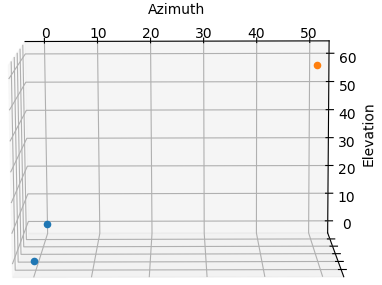
\includegraphics[width=0.98\textwidth]{Figures/2mic1src.png}
%    \caption{Figure depicts a source located at $50\degree$ azimuth and $60\degree$ elevation (orange dot). Two microphones (blue dots) will be used to localize the source.}
%    \label{fig:2mic1srcPos}
%\end{figure}
\begin{figure}[H]
    \centering
    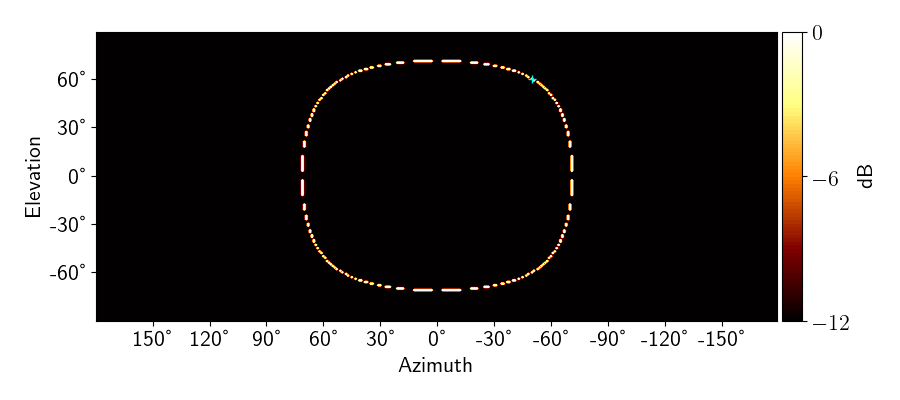
\includegraphics[width=0.8\textwidth]{Figures/2mic1srcRes.png}
    \caption{SRP-PHAT is run to localize a single point source using two microphones $M_{1} and M_{2}$ as described in appendix \ref{app:micLocs}. The source can only be localized to a circle. The blue cross in the figure indicates the actual source location. Note that the reason the circle does not appear exactly circular in image is due to the cylindrical projection being used to display the result.}
    \label{fig:2mic1src}
\end{figure}
The results in Fig. \ref{fig:2mic1src} are displayed using the cylindrical projection technique, such that the entire spherical space around the origin can be shown as a rectangle, with x-axis being the azimuth and y-axis being the elevation. This technique is employed throughout the thesis to give a full picture of the localization results.

A new circle will result for each new microphone pair used to localize the source, as long as the microphone pairs are not all placed in the same line\footnote{In the case of a linear array, the multiple circles would overlap completely}. For example, for three microphones A, B and C placed in an equilateral triangle formation, three circles can be computed (one each for AB, BC and CA). The maximum peak occurs at 2 locations with (-50$\degree$,$\pm$ 60$\degree$) as shown in Fig. \ref{fig:3mic1src}. If a fourth microphone is placed in the same plane as the triangle, the array response will be a combination of circles from 6 possible microphone pairs ($^4C_2$). However, the new circles would all pass through the same 2 locations. For a non co-planar array, e.g. a tetrahedral array, the maximum peak occurs at exactly one poin, shown in \ref{fig:4mic1src}. 
\subsection{Some considerations with SRP-PHAT}
\subsubsection{Subsidiary peaks}
Even though a tetrahedral array is able to detect a point source to a single maximum peak position, subsidiary peaks can appear in the energy map at DOAs that don't correspond to the true source DOA, since, the cross-correlations values at computed delays are summed by the beamformer (Eq. \ref{eq:srpSum}). For example, points where only 2-5 of the circles meet. If multiple sources are localized, these peaks in the SRP-PHAT energy map can add up leading to the detection of a fake source and can also mask real sources. The effect of these subsidiary peaks can be reduced by increasing the number of microphones. This is because, even though more microphone pairs would mean more localization circles, it also means the real peaks would be higher, effectively lowering the noise/subsidiary peak floor. Indeed, solutions in the market exist with even 90 microphones (\cite{batel2003noise}, Fig. 31). However, since, the number of microphones is a constraint requirement for this thesis, this solution is not considered.
\subsubsection{Linear dependency}
Since only 3 pairs out of the 6 in a tetrahedral array are linearly independent (Eq. \ref{Eq:linearDep}), the localization can also be done considering only 3 of those pairs. The result in shown in Fig. \ref{fig:4mic1srcInd}.
\begin{figure}[!ht]
    \centering
    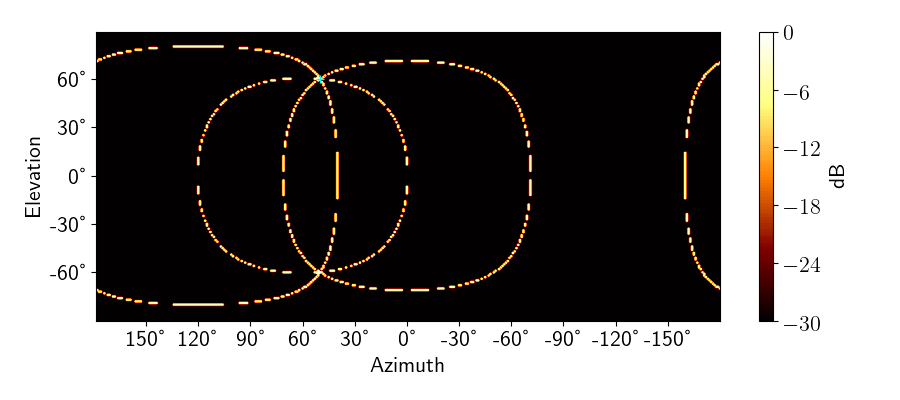
\includegraphics[width=0.8\textwidth]{Figures/3mic1srcRes.png}
    \caption{SRP-PHAT is run to localize the source with 3 microphones $M_{1}, M_{2} and  M_{3}$ as described in appendix \ref{app:micLocs}.}
    \label{fig:3mic1src}
\end{figure}
\begin{figure}[!ht]
    \centering
    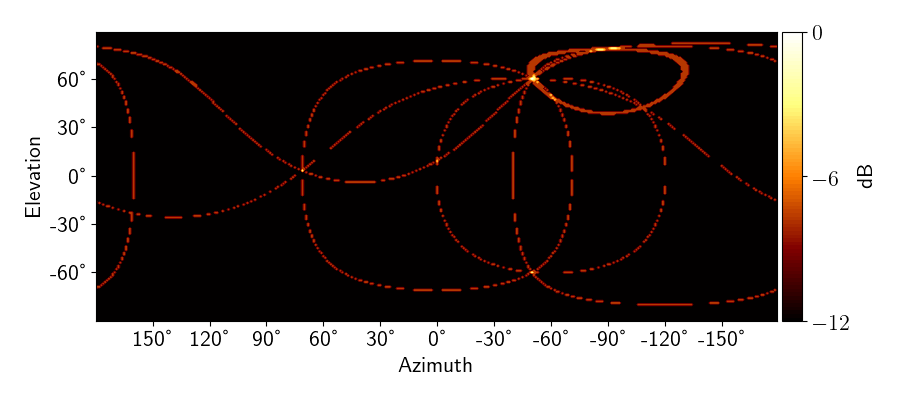
\includegraphics[width=0.8\textwidth]{Figures/4mic1srcRes.png}
    \caption{SRP-PHAT is run to localize the source with a tetrahedral array ($M_{1}, M_{2},  M_{3} and M_{4}$ as described in appendix \ref{app:micLocs}).}
    \label{fig:4mic1src}
\end{figure}
\begin{figure}[!ht]
    \centering
    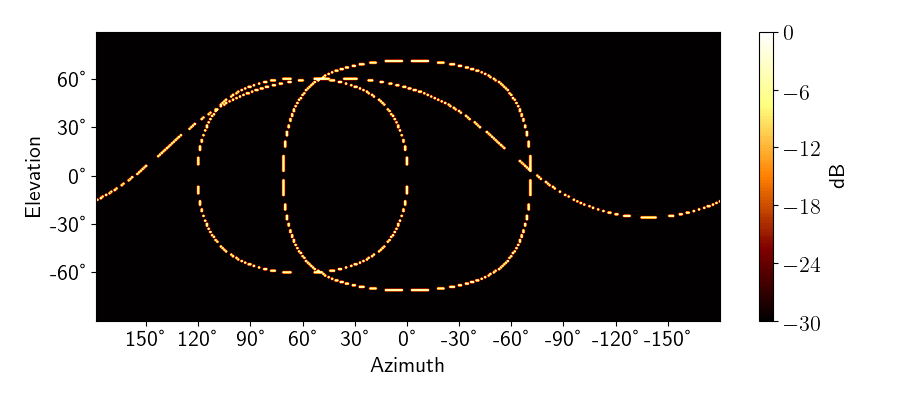
\includegraphics[width=0.8\textwidth]{Figures/Ind4mic1srcRes.png}
    \caption{SRP-PHAT is run to localize the source with a tetrahedral array but only linearly independent microphone pairs are considered}
    \label{fig:4mic1srcInd}
\end{figure}
Considering only independent microphones, Eq. \ref{eq:srpSum} can be rewritten as,
\begin{equation}
    S_{SRP}(\theta,\phi)=\sum\limits_{i=1}^{M-1}{R_{x_0,x_i}[f_{0,i}(\theta,\phi)]}
     \label{eq:srpSumInd}
\end{equation}
%\subsection{Using the redundant information from the microphone pairs}
The thing to note is that Eq. \ref{Eq:linearDep} is only true for no noise conditions. In noisy conditions, there is a potential to gain information by using the redundant microphone pairs. This is because if noise at all microphones is assumed to be uncorrelated, then even though the noise causes certain microphone pairs to detect a source at a `sourceless' location, other microphone pairs might detect a lower magnitude at that location. Due to more microphone pairs, the sum of all microphone pairs will be even higher at the real source location, and at other locations, the sum due to the noise will be suppressed. It can be seen in Fig. \ref{fig:4mic1src} that using all the microphone pairs adds to the overall noise on the map as more pairs can now contribute to the SRP sum, leading to more circles. However, the peak of the true source also becomes higher, due to more pairs providing power at the source location. This means that even though the noisy floor is has noise in more locations, it is of a lower magnitude, leading to a higher achievable dynamic range. For this reason, from here on the localization results considers all possible pair of microphones.
